\documentclass{beamer}
\usepackage{appendixnumberbeamer}
\usepackage{graphicx}
\usepackage{natbib}
\usepackage{mathtools}
\usepackage[absolute,overlay]{textpos}
\usepackage{outlines}
\usepackage{minted}


\setbeamercolor{alerted text}{fg=black}
\setbeamerfont{alerted text}{series=\bfseries}

\newcommand\mycite[1]{%
  \begin{textblock*}{5cm}(.7\textwidth,9cm)%
    #1
  \end{textblock*}
}



\bibliographystyle{apj.bst}

\usetheme{Madrid}
\setbeamertemplate{navigation symbols}{}
\setbeamertemplate{footline}{}

\AtBeginSection[]
{
  \begin{frame}
    \frametitle{Table of Contents}
    \tableofcontents[currentsection]
  \end{frame}
}

\begin{document}

\title{SIMPLE-ABC: \\ Statistical Inference for Multiple PLanet systems Employing Approximate Bayesian Computation }  
\author{Robert C. Morehead}
\date{04/30/2014} 
\institute[Penn State]{The Pennsylvania State University}



\begin{frame}[plain]
\begin{center}

\includegraphics{mark2tonesolid.eps}
\end{center}
\titlepage
\end{frame}



%\section{Project 2: SIMPLE-ABC}
%\subsection{Motivation}
\begin{frame}{We would like to make inferences about the underlying distribution(s) of \emph{Kepler} Planets.}
\mycite{\cite{Fang:2012}}
\begin{columns}[c] 
\begin{column}[T]{4cm}
-What is the  number of planets per star? \\ 
\vspace{0.5cm}
-What is the distribution of mutual inclinations? \\
\vspace{0.5cm}
-What is the distribution of planet eccentricities? \\


\end{column}
\begin{column}[T]{6cm}
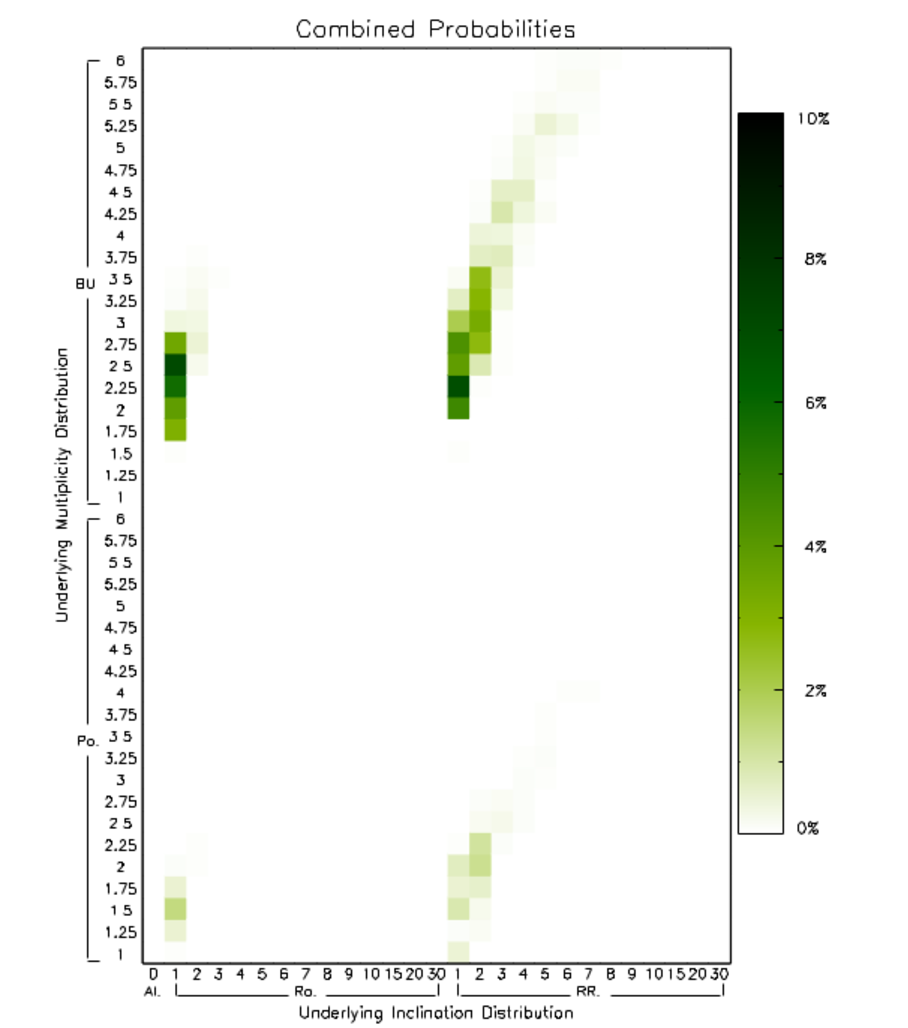
\includegraphics[scale=.35]{fang.pdf}
\end{column}
\end{columns}
\end{frame}

\begin{frame}{We want to infer the posterior probability of some
 model with parameters $\theta$. }
\begin{center}
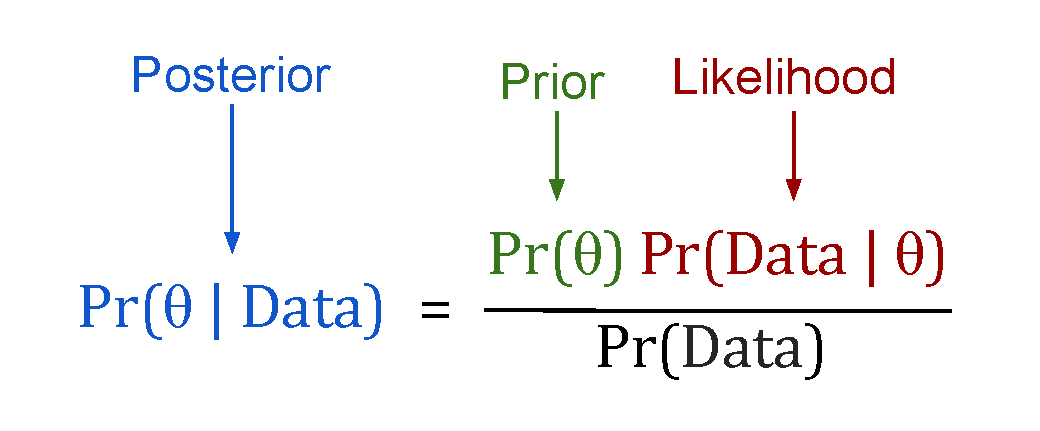
\includegraphics[scale=.65]{Bayes_theorem.pdf}
\end{center}
\end{frame}

%\subsection{ABC Overview}
\begin{frame}{Approximate Bayesian Computation (ABC) is a likelihood-free method to infer posterior distributions.}
\begin{center}
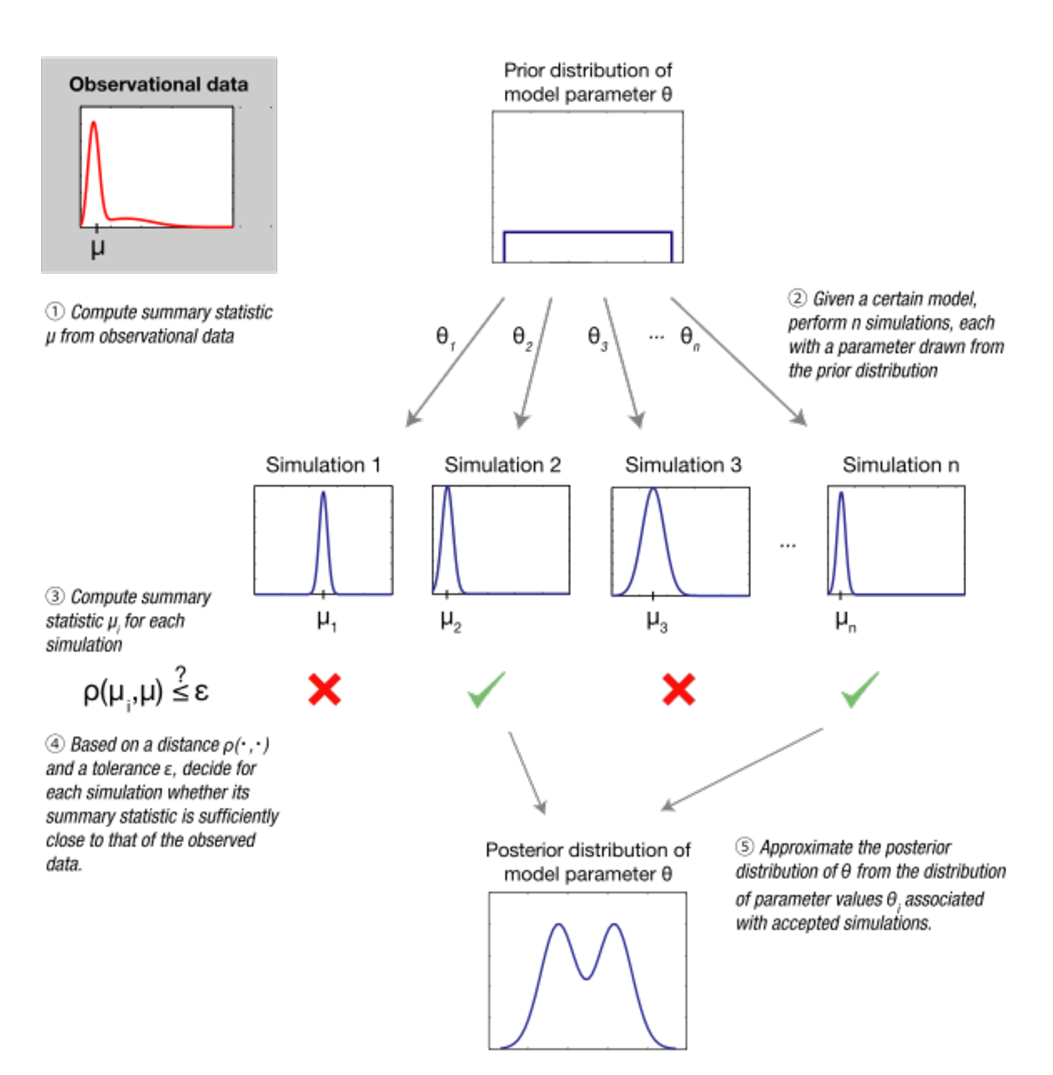
\includegraphics[scale=.38]{ABC.pdf}
\end{center}
\mycite{\cite{Sunnaker:2013}}
\end{frame}


\begin{frame}[fragile]{I took an object-oriented approach using Python.}
\tiny
\begin{minted}[linenos=true]{python}
class Model(object):

    def __call__(self, theta):
        return self.generate_data_and_reduce(theta)

    def set_data(self, data):
            self.data = data
            self.data_sum_stats = self.summary_stats(self.data)

    def generate_data_and_reduce(self, theta):
        """
        A combined method for generating data, calculating summary statistics
        and evaluating the distance function all at once.
        """
        synth = self.generate_data(theta)
        sum_stats = self.summary_stats(synth)
        d = self.distance_function(sum_stats, self.data_sum_stats)
        return d

    def draw_theta(self):
        raise NotImplementedError('You must override the draw_theta '
                                  'method in your own subclass.')

    def generate_data(self, theta):
        raise NotImplementedError('You must override the generate_data '
                                  'method in your own subclass.')

    def summary_stats(self, data):
        raise NotImplementedError('You must override the summary_stats '
                                  'method in your own subclass.')

    def distance_function(self, summary_stats, summary_stats_synth):
        raise NotImplementedError('You must override the distance_function '
                                  'method in your own subclass.')
\end{minted}
\end{frame}




\begin{frame}{For testing purposes, I implemented two models.}
\begin{center}
\begin{columns}[c] 
\begin{column}[T]{5cm}
\textbf{Normal Distribution}  \\
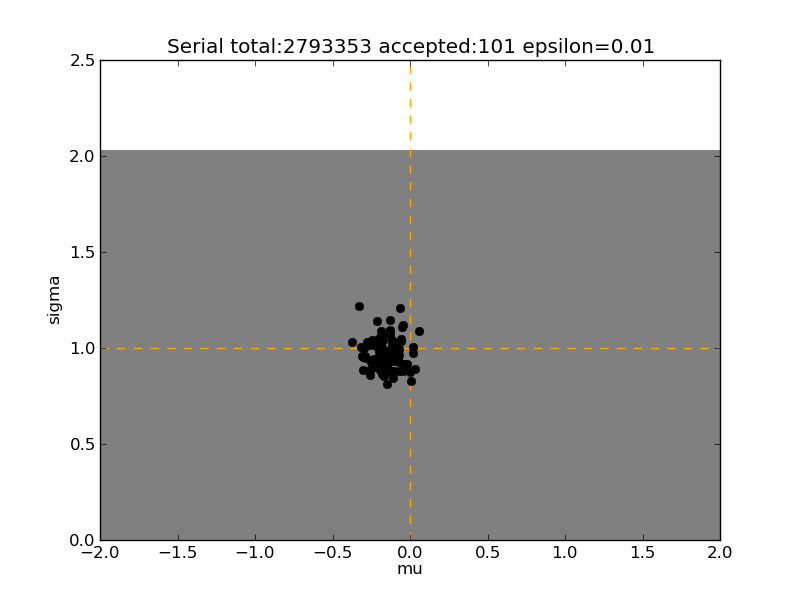
\includegraphics[scale=.27]{Serialnorm.png}
\end{column}
\begin{column}[T]{5cm}
 \textbf{Simple Planet Model} \\
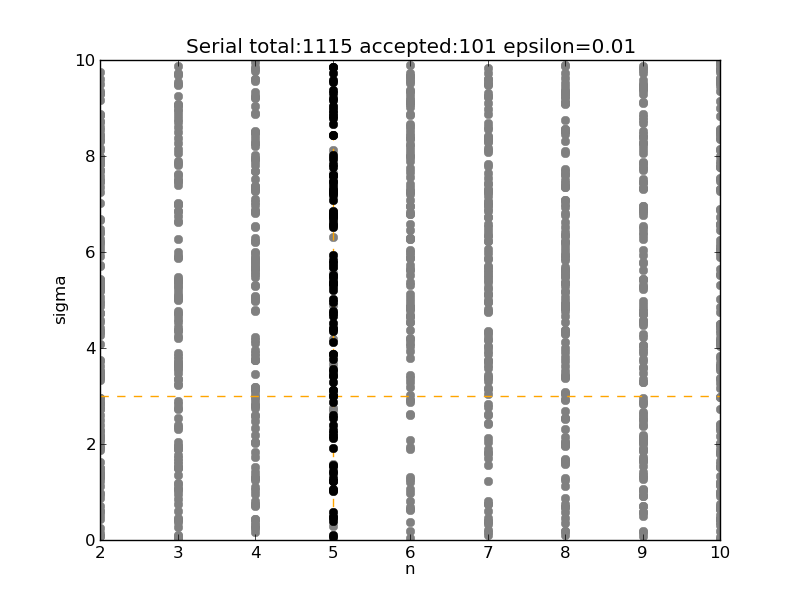
\includegraphics[scale=.27]{Serial.png}
\end{column}
\end{columns}
\end{center}
\end{frame}


\begin{frame}{Parallelization via multiprocessing.pool.map works pretty well...}
\begin{center}
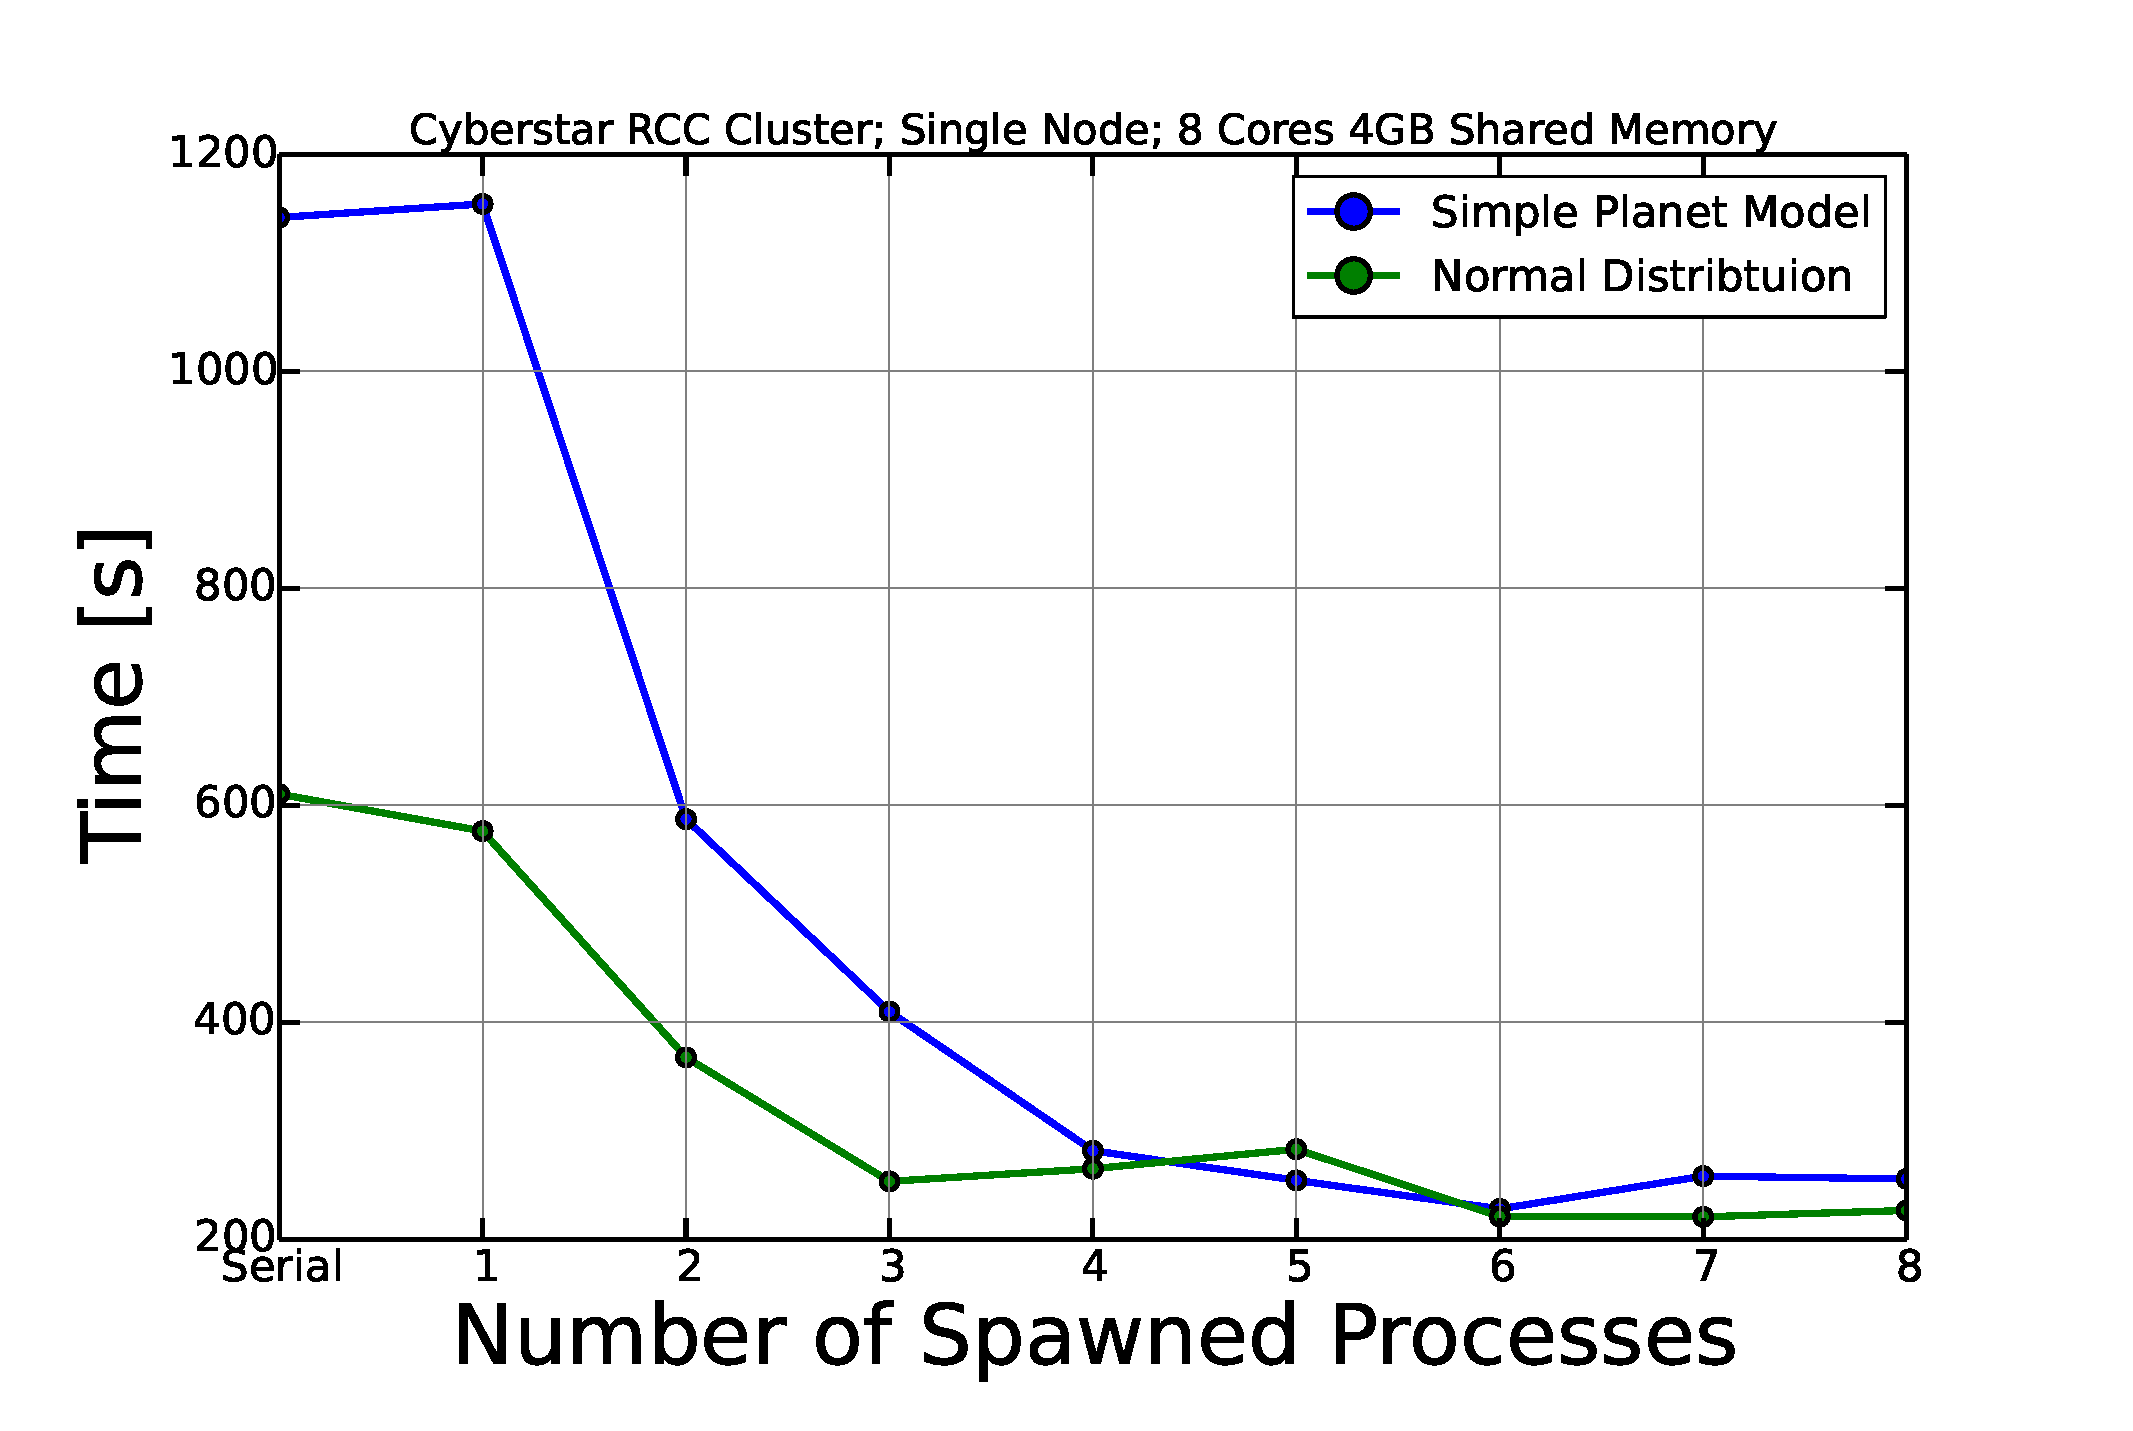
\includegraphics[scale=.3]{time.eps}
\end{center}
\end{frame}

\begin{frame}{and even better for complex models!}
\begin{center}
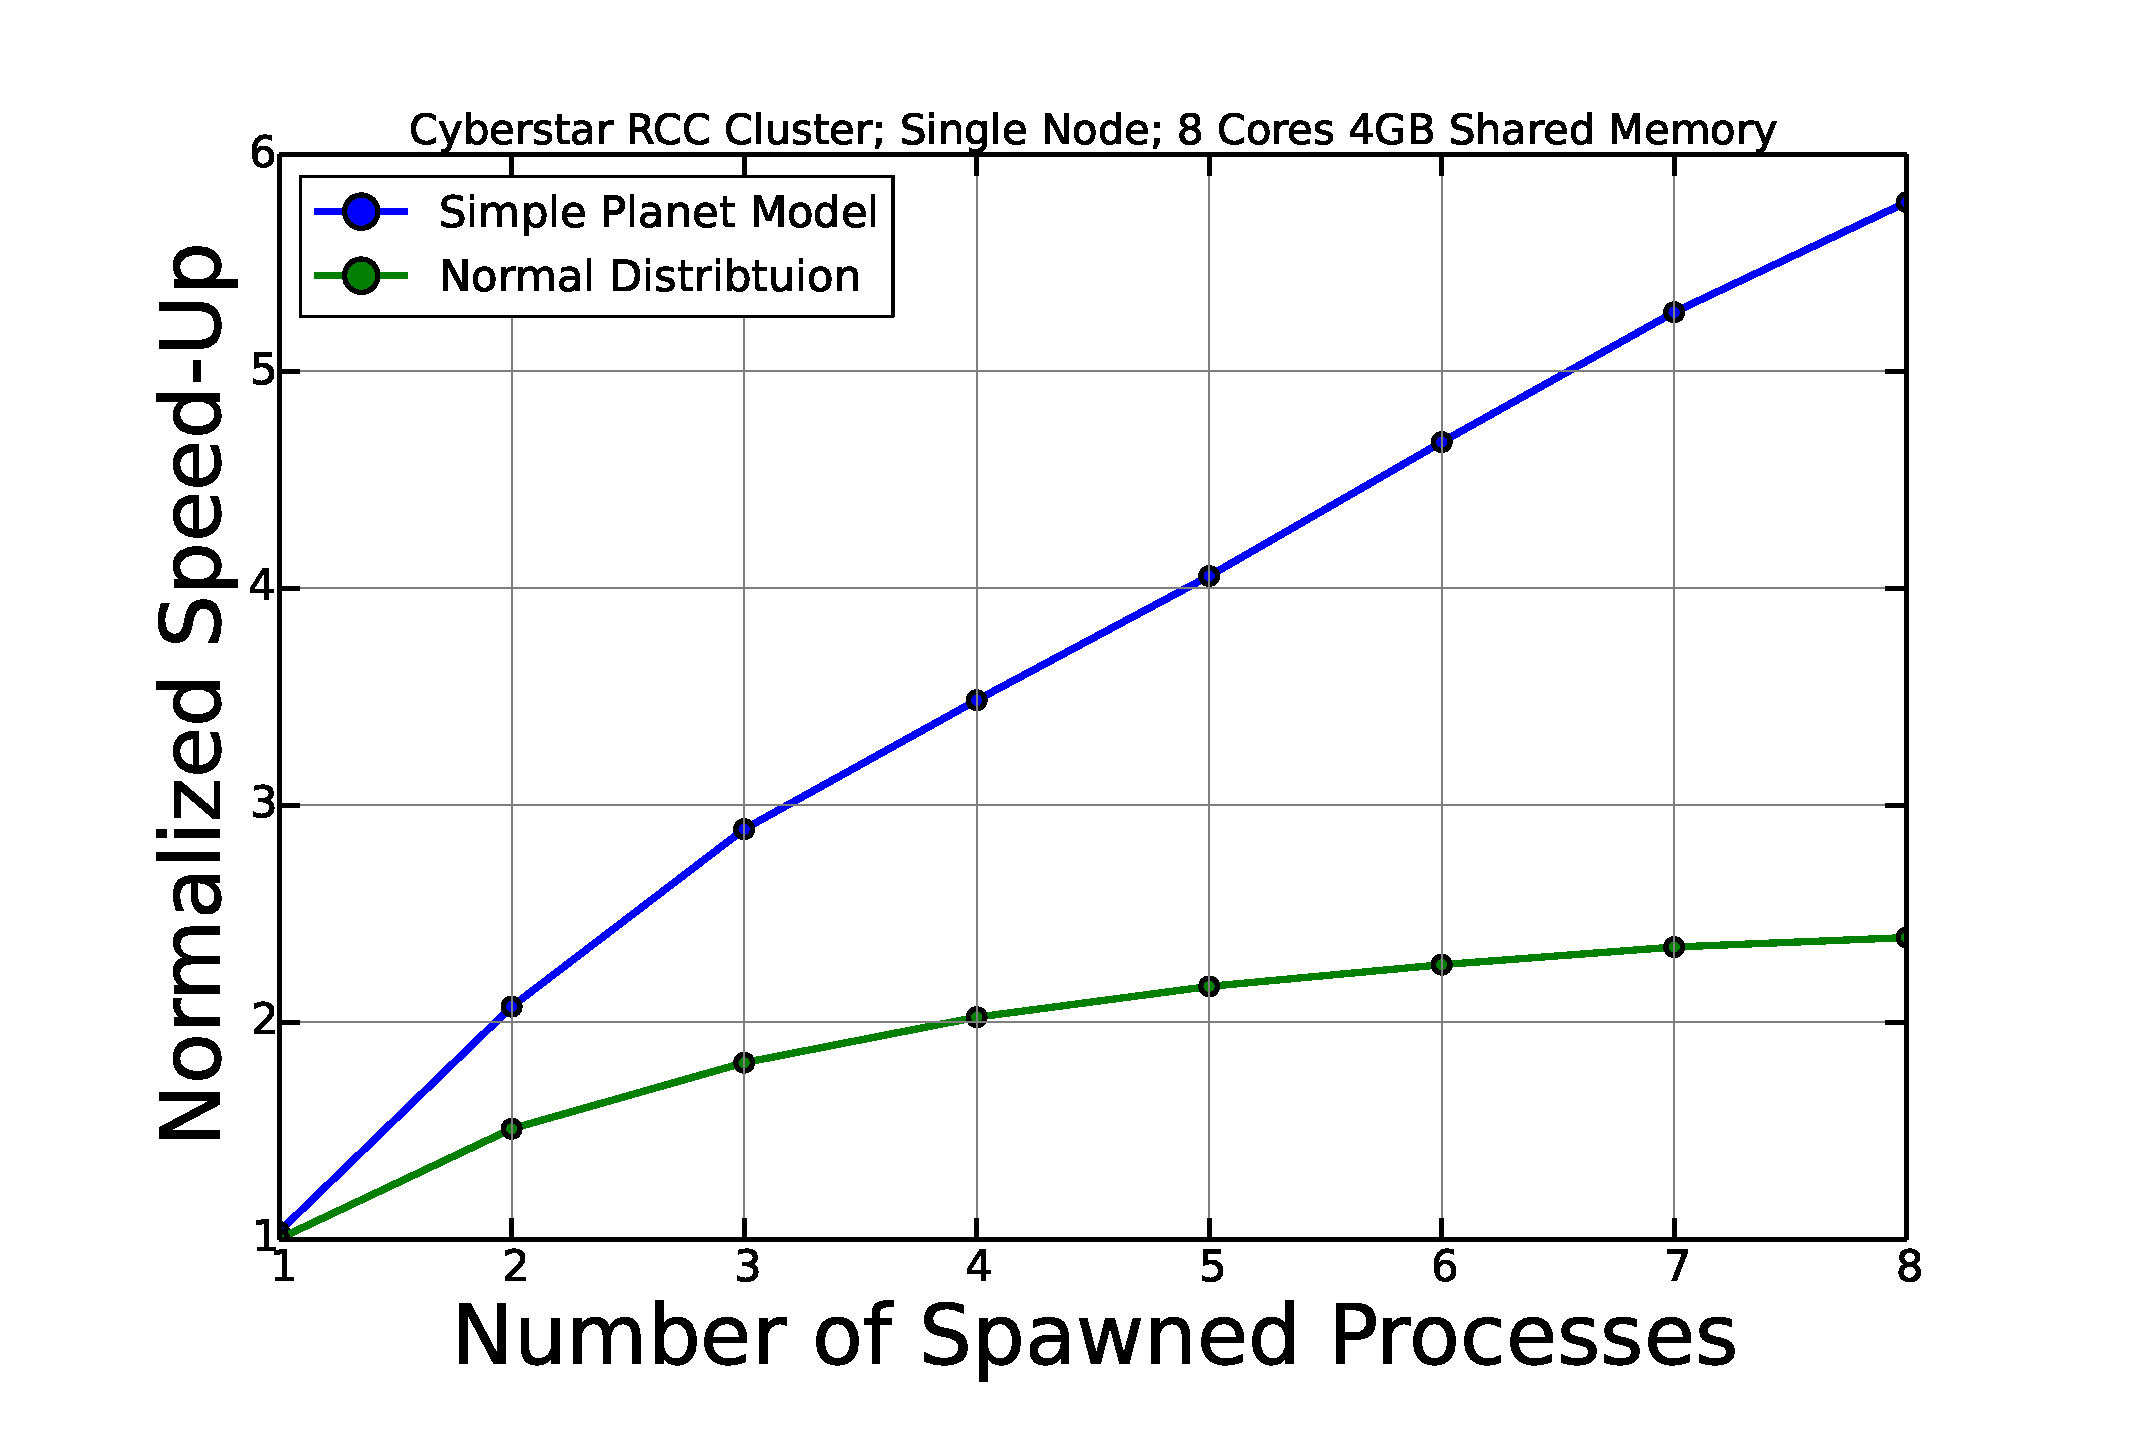
\includegraphics[scale=.3]{speedup.eps}
\end{center}
\end{frame}

\begin{frame}{I tried cloud computing with Domino Data Labs.}
\begin{center}
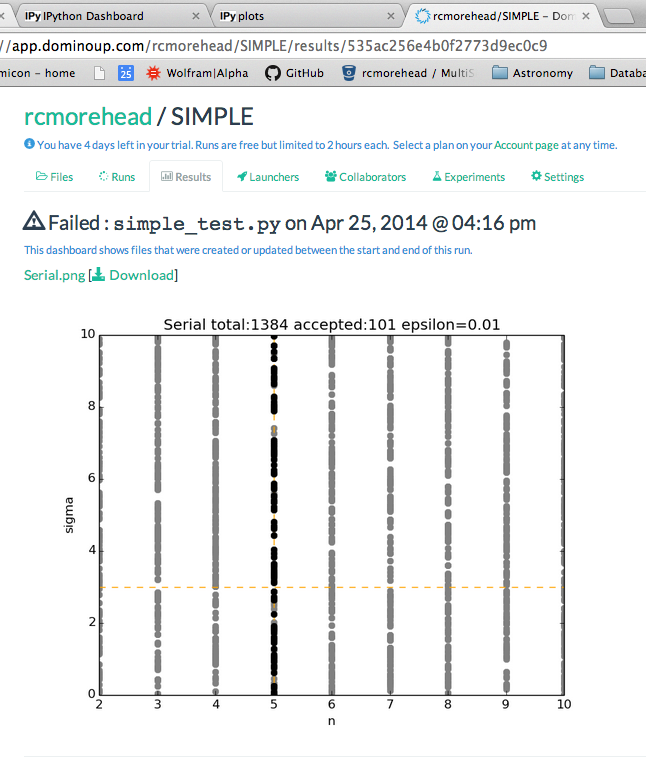
\includegraphics[scale=.27]{domino.png}
\end{center}
\end{frame}

\begin{frame}{If I had presented on Monday, that would have been it...}
\begin{center}
\includegraphics[scale=.3]{time-c.eps}
\end{center}
\end{frame}

\begin{frame}{The gains in performance are \emph{almost} as good.}
\begin{center}
\includegraphics[scale=.3]{speedup-c.eps}
\end{center}
\end{frame}

\begin{frame}{But in the cloud system does not scale quite as well.}
\begin{center}
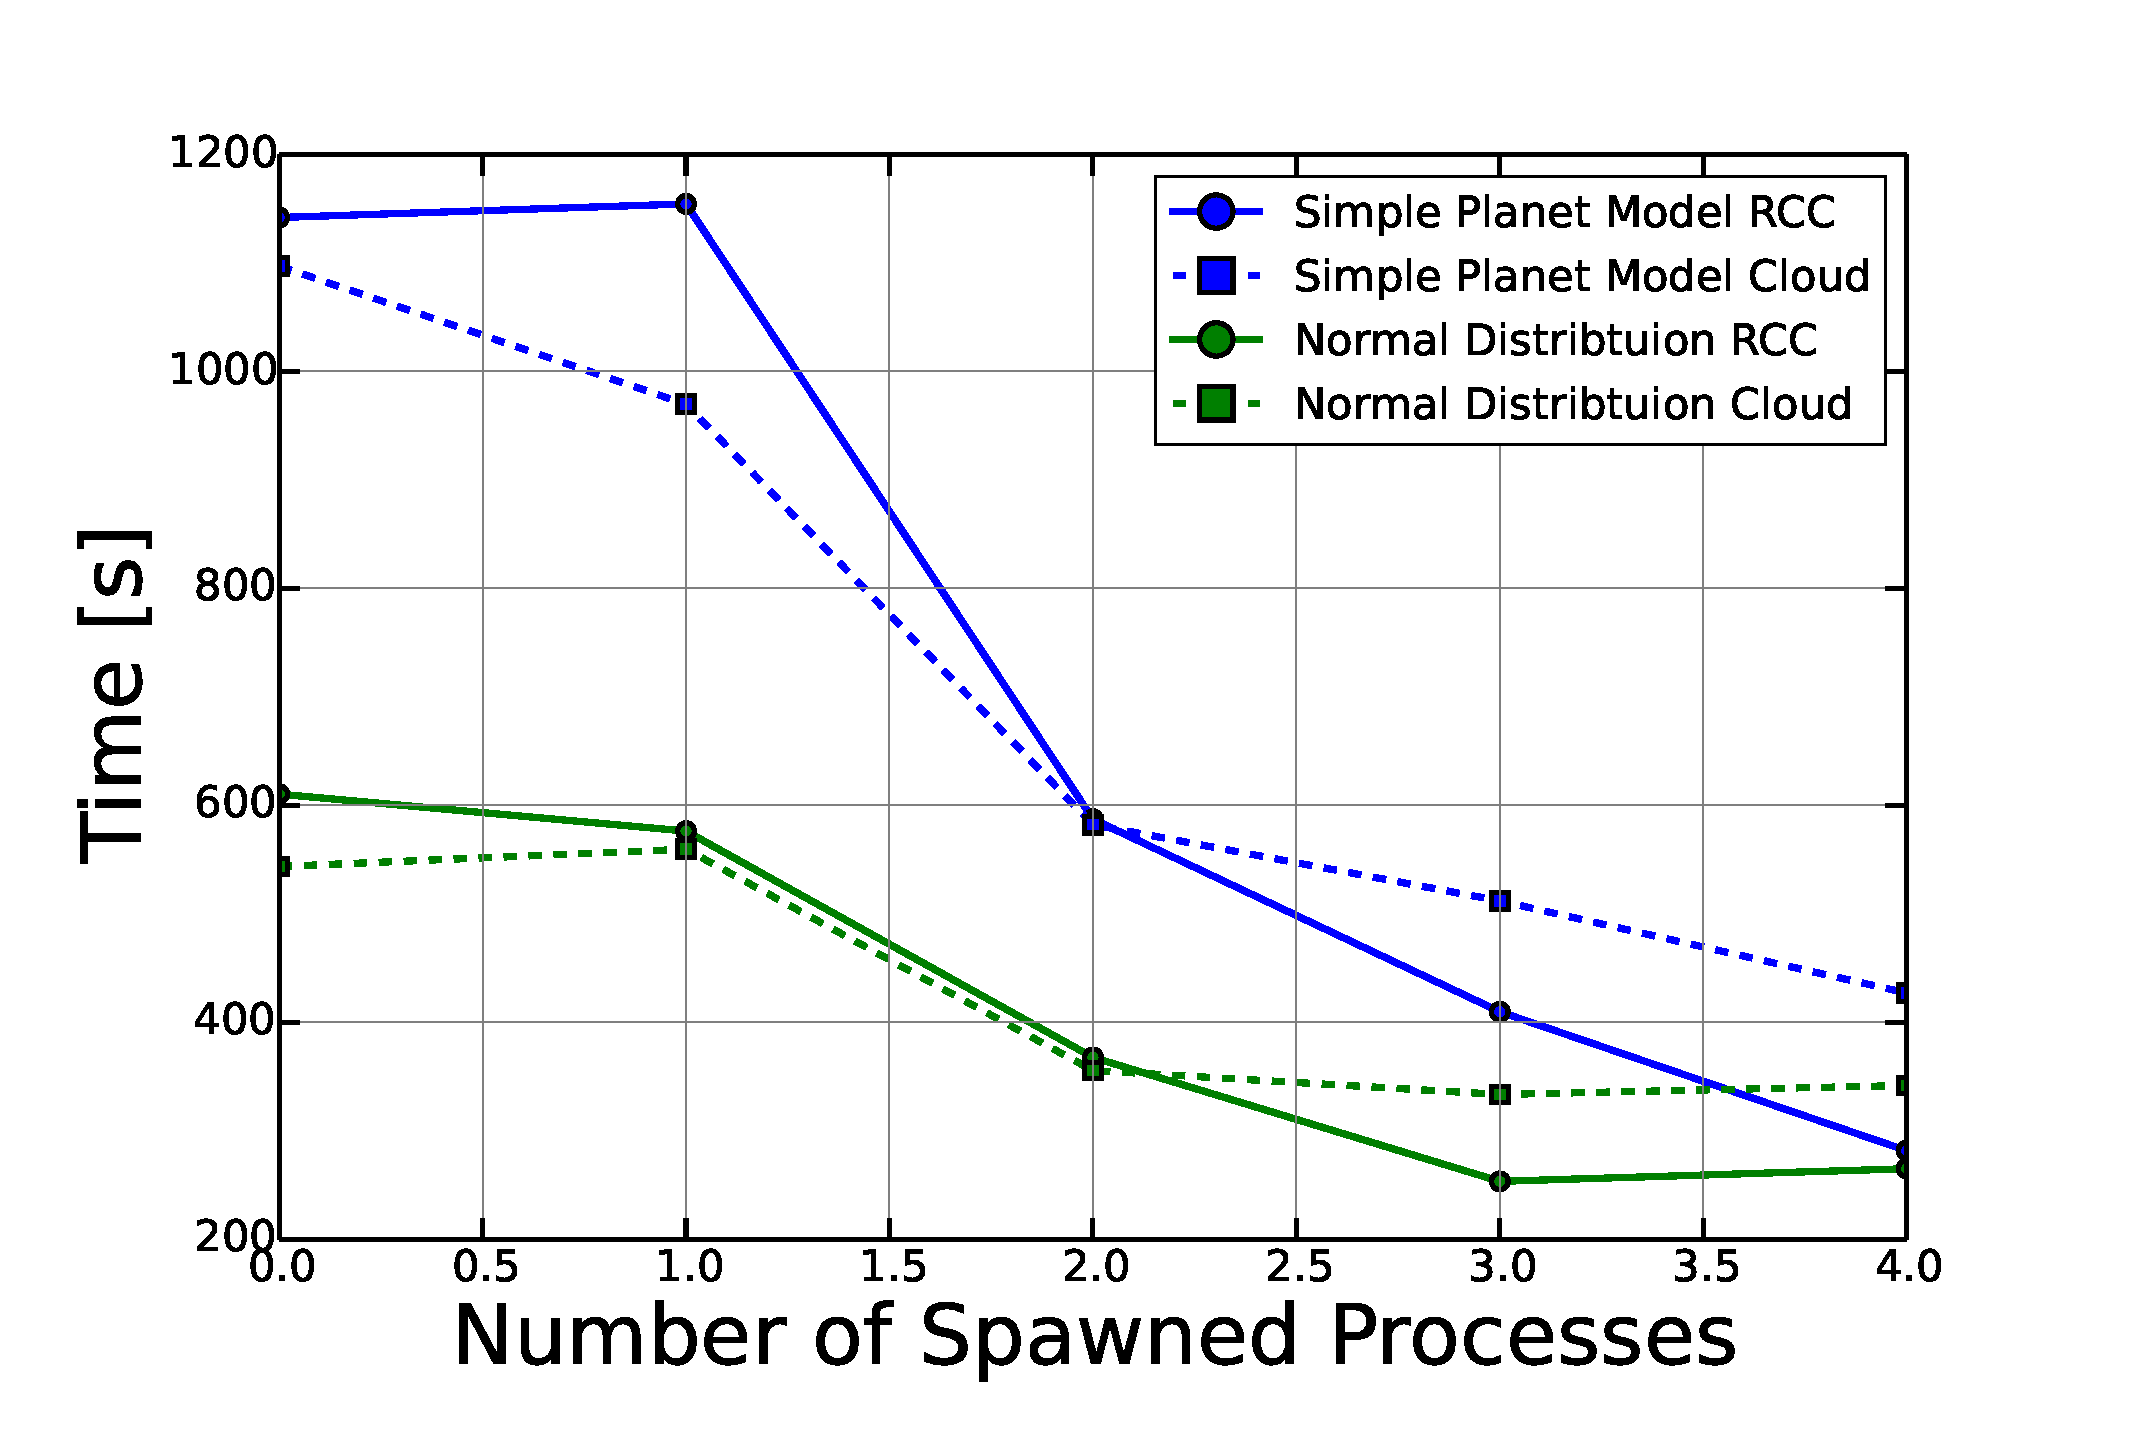
\includegraphics[scale=.3]{time-vs.eps}
\end{center}
\end{frame}

\begin{frame}{But in the cloud system does not scale quite as well.}
\begin{center}
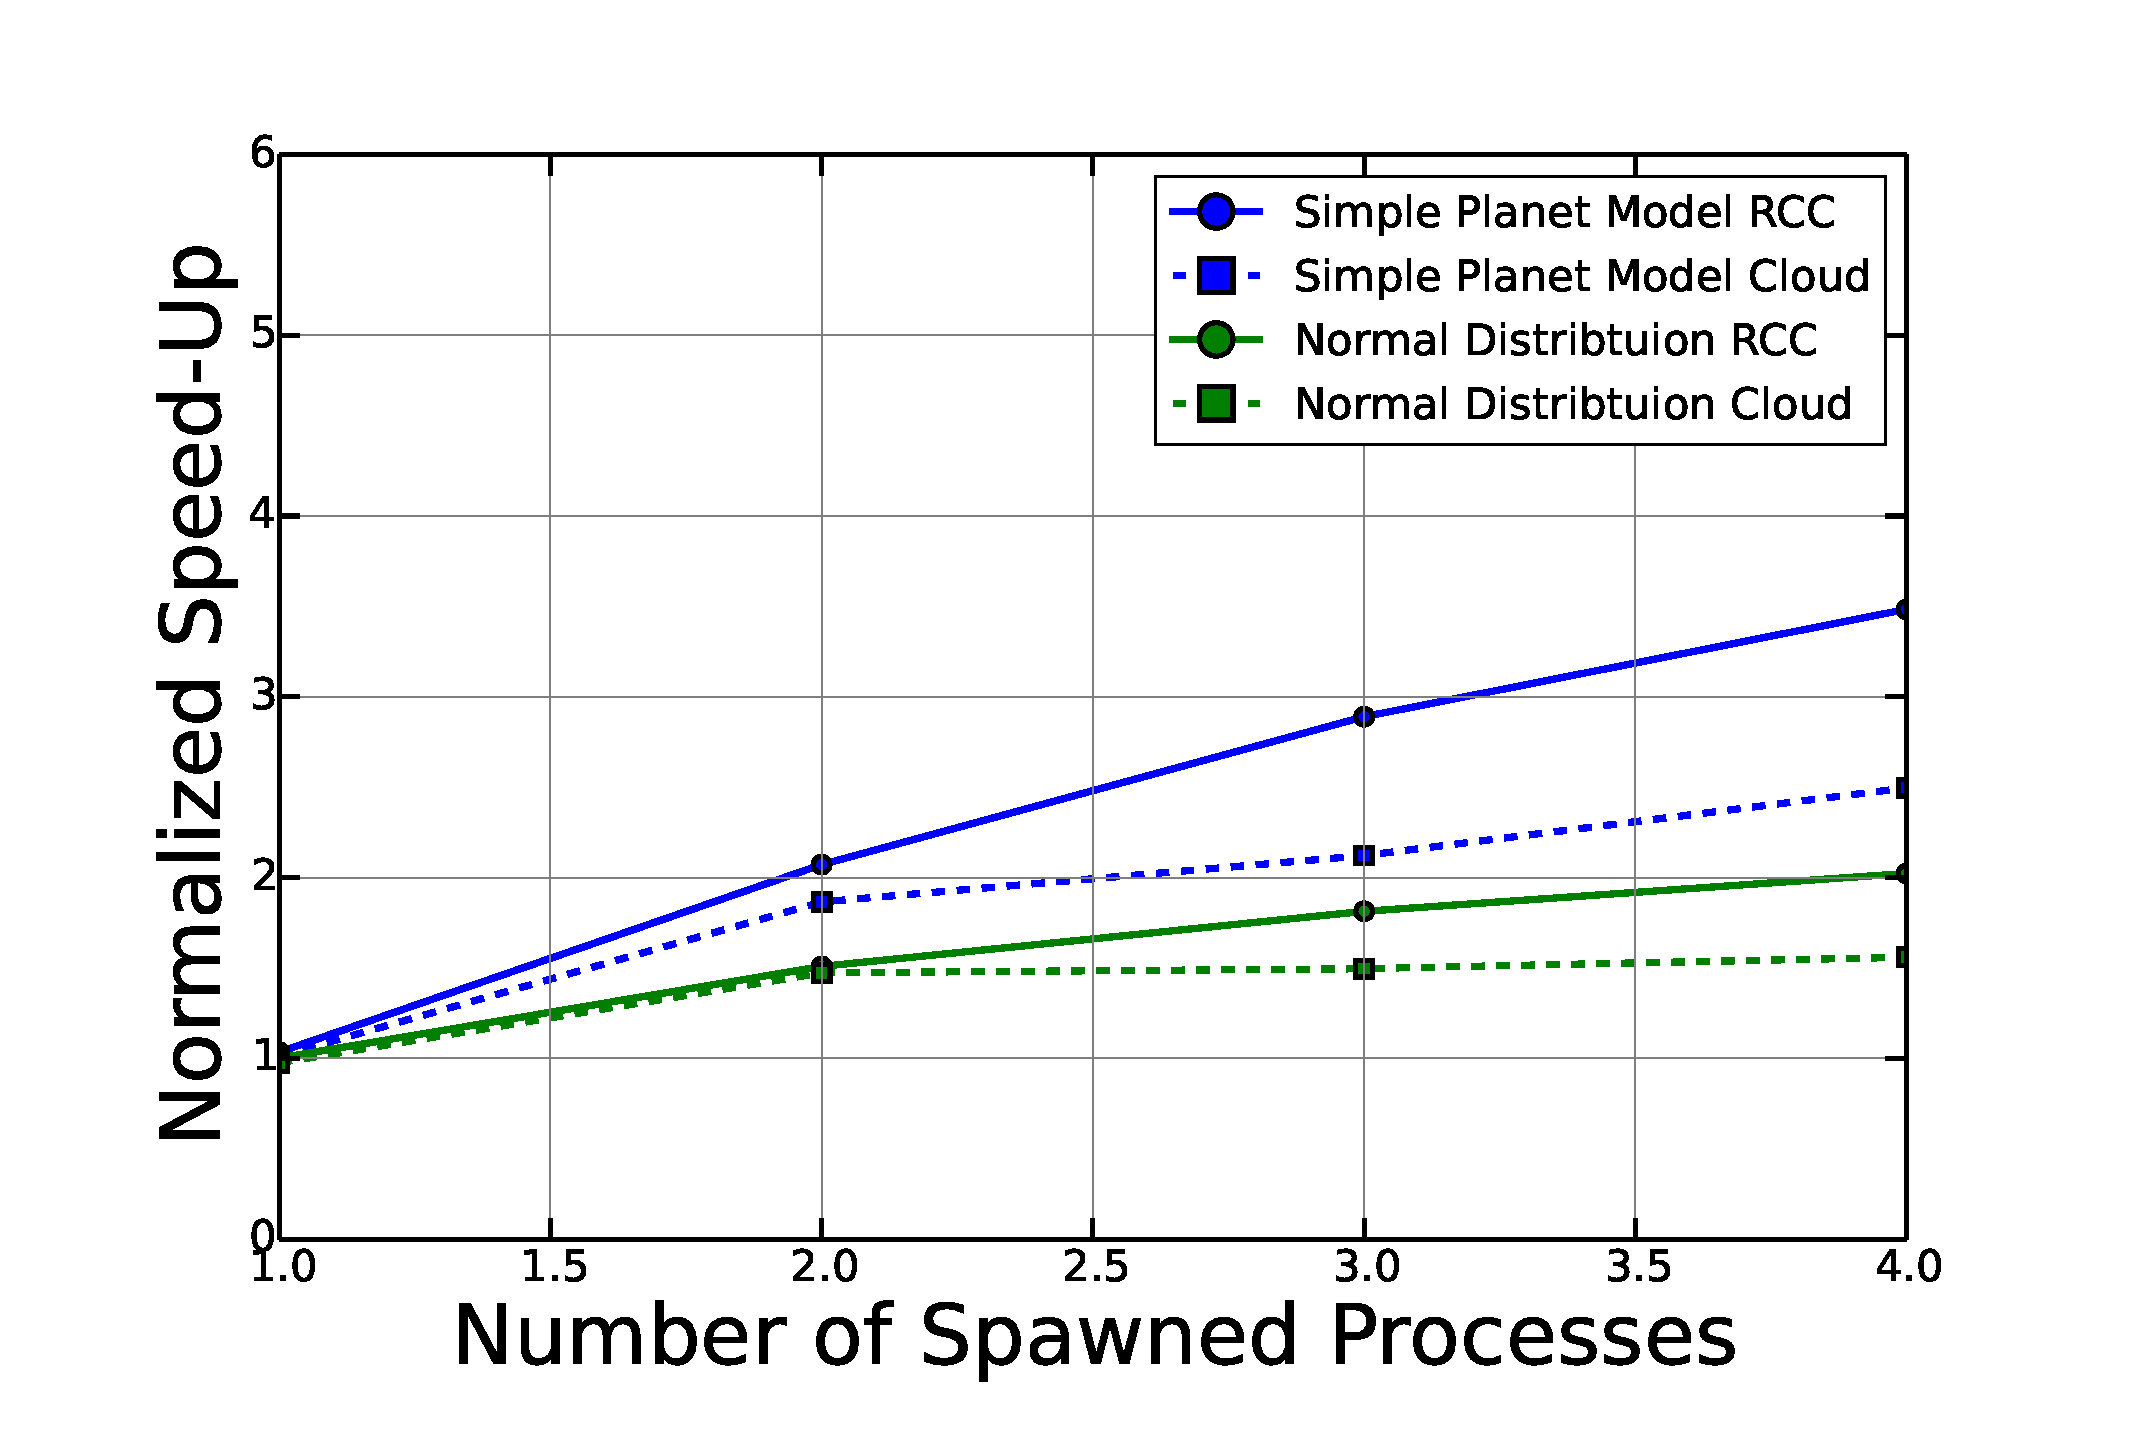
\includegraphics[scale=.3]{speedup-vs.eps}
\end{center}
\end{frame}


\begin{frame}[plain]
\begin{center}

\includegraphics{mark2tonesolid.eps}
\Huge
The End
\end{center}
\end{frame}

\begin{frame}[plain]
\begin{center}
\Huge
Nothing to see here!
\end{center}
\end{frame}


\appendix


\begin{frame}{For testing purposes, I implemented two models.}
\begin{center}
\begin{columns}[l] 
\begin{column}[T]{5cm}
\textbf{Normal Distribution}  \\
\vspace{0.5cm}
$\theta = (\mu,\sigma)$ \\
\vspace{0.5cm}
$(\mu=0, \sigma=1)$ \\
\vspace{0.5cm}
$\widehat{S} =$ (25th, 75th percentiles) \\
\vspace{0.5cm}
$D = \sqrt{\widehat{S}_{0}^2 + \widehat{S}_{1}^2 }$ \\
\vspace{0.5cm}
$\epsilon = 0.01$ \\
\vspace{0.5cm}
Minimum particles = 100
\vspace{0.5cm}


\end{column}
\begin{column}[T]{5cm}
 \textbf{Simple Planet Model} \\
 \vspace{0.5cm}
 $\theta = (n,\sigma)$ \\
 \vspace{0.5cm}
$(n=5, \sigma=3)$ \\
\vspace{0.5cm}
$\widehat{S} =$ (N transits per star, $b$) \\
\vspace{0.5cm}
$D = \sqrt{D_{KS}(\widehat{S}_{0})^2 + D_{KS}(\widehat{S}_{1})^2 }$ \\
\vspace{0.5cm}
$\epsilon = 0.01$ \\
\vspace{0.5cm}
Minimum particles = 100
\vspace{0.5cm}
\end{column}
\end{columns}
\end{center}
\end{frame}

\begin{frame}{}
\bibliography{master}
\end{frame}
\end{document}
